\subsubsection{Snapshot service}
This component is responsible of taking snapshots.

We show in figure \ref{fig:mw-snapshot} the architecture of this service and
then we will show in detail each module that composes this component.

\begin{figure}[H]
  \centering
  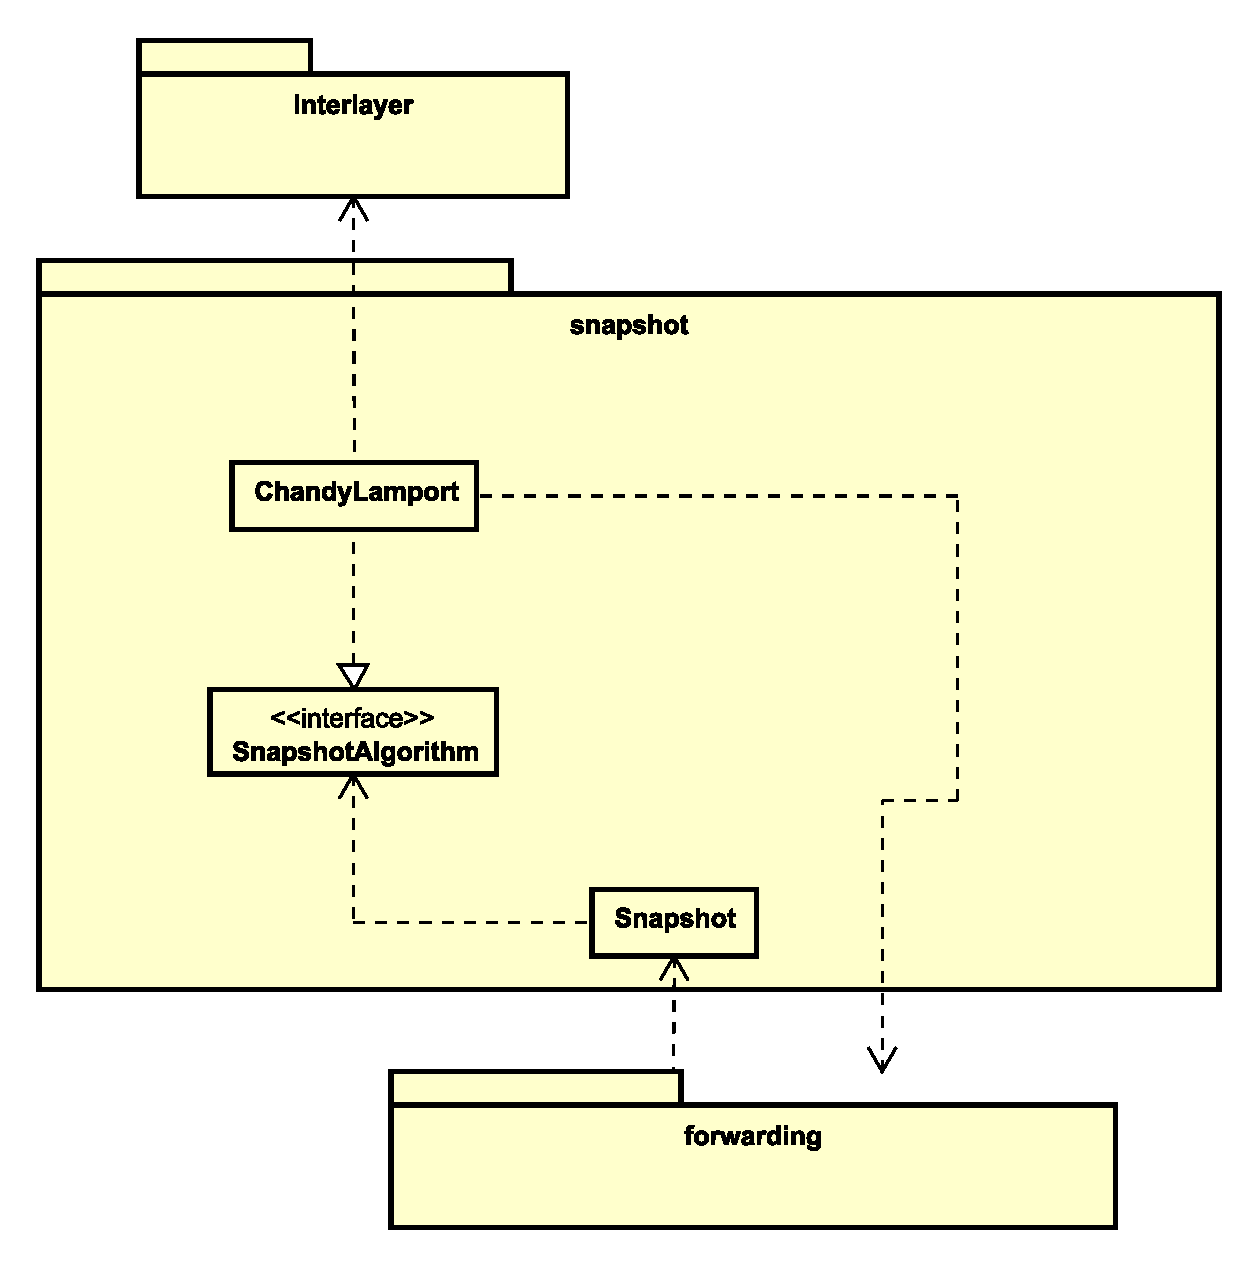
\includegraphics[width=\columnwidth]{images/solution/mw/snapshot.eps}
  \caption{Middleware's Snapshot service}
  \label{fig:mw-snapshot}
\end{figure}

\subsubsubsection{snapshot.Snapshot}

\begin{figure}[H]
  \centering
  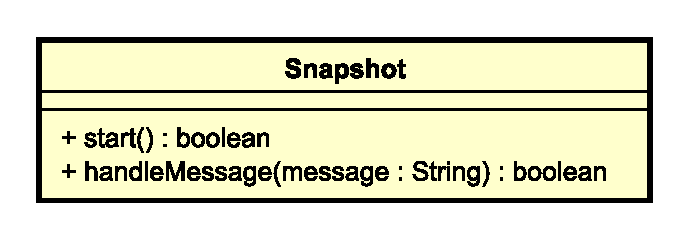
\includegraphics[width=.5\columnwidth]{images/solution/mw/sn/snap.eps}
  \caption{snapshot.Snapshot}
  \label{fig:mw-snapshot-snapshot}
\end{figure}

\FloatBarrier
\begin{itemize}
  \item \textbf{Description} \\
    This module is the Fa\c cade of the Snapshot service. It is responsible
    to boot neatly and supervise all processes in Snapshot. Also, it has to
    handle snapshot requests that come from other nodes of the system.
  \item \textbf{Attributes}
  \item \textbf{Operations}
  \begin{itemize}
    \item \texttt{+ start()} \\
    Starts the Snapshot service.
    \item \texttt{+ handleMessage(message: String)} \\
    % TODO: check this out: Message will really be a String?
    Handles a snapshot start/termination request that comes from other nodes
    or receives snapshot information from the application layer.
  \end{itemize}
\end{itemize}

\subsubsubsection{snapshot.SnapshotAlgorithm}

\begin{figure}[H]
  \centering
  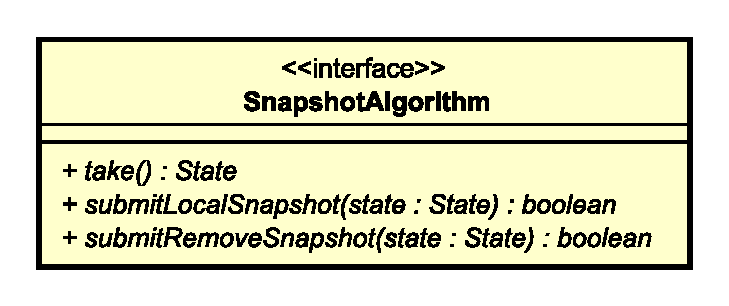
\includegraphics[width=.5\columnwidth]{images/solution/mw/sn/snalg.eps}
  \caption{snapshot.SnapshotAlgorithm}
  \label{fig:mw-snapshot-snapshotalgorithm}
\end{figure}
    % TODO: define State type

\FloatBarrier
\begin{itemize}
  \item \textbf{Description} \\
    Interface for processes that implement a certain kind of snapshot.
  \item \textbf{Attributes}
  \item \textbf{Operations}
  \begin{itemize}
    \item \texttt{+ take()} \\
    Starts to take a snapshot.
    \item \texttt{+ submitLocalSnapshot(state : State)} \\
    Stores a local snapshot.
    % TODO: define State type
    \item \texttt{+ submitRemoteSnapshot(state : State)} \\
    Stores a remote snapshot.
    % TODO: define State type
  \end{itemize}
\end{itemize}

\subsubsubsection{snapshot.ChandyLamport}

\begin{figure}[H]
  \centering
  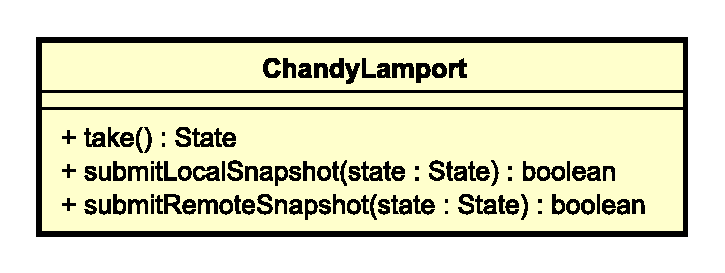
\includegraphics[width=.5\columnwidth]{images/solution/mw/sn/sncl.eps}
  \caption{snapshot.ChandyLamport}
  \label{fig:mw-snapshot-chandylamport}
\end{figure}
    % TODO: define State type

\FloatBarrier
\begin{itemize}
  \item \textbf{Description} \\
    Module that implements the \texttt{snapshot.SnapshotAlgorithm}
    interface to take snapshots with the algorithm by Chandy and Lamport.
  \item \textbf{Attributes}
    % TODO: Add list of states?
  \item \textbf{Operations}
  \begin{itemize}
    \item \texttt{+ take()} \\
    Starts to take a snapshot: that implies Forwarding module to notify
    other nodes of that and to hold messages until the snapshot is over; also
    that implies Interlayer to issue a snapshot request to the application
    layer.
    \item \texttt{+ submitLocalSnapshot(state : State)} \\
    Stores the snapshot of the node where the process is executing.
    % TODO: define State type
    \item \texttt{+ submitRemoteSnapshot(state : State)} \\
    Stores the snapshot of a remote node.
    % TODO: define State type
  \end{itemize}
\end{itemize}
